% ----------------------------------------------------------------------------
% DSP
% ----------------------------------------------------------------------------

\chapter{Processamento de Sinais Digitais}

Enfim chegamos no processamento de áudio propriamente dito: \emph{Digital
Signal Processing} ou processamento de sinal digital.
O Pure Data possui inlets e outlets específicos para o processamento de sinal.
É fácil reconhecer: eles são pintados de cinza escuro.
Além disto, classes que operam com processamento de sinal e que possuem iolets
DSP costumam ser nomeadas \texttt{class~}.

\begin{figure}[h!]
\centering
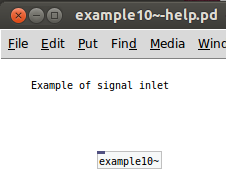
\includegraphics[scale=\Mysize]{example10}
\caption{Primeiro Inlet DSP}
\end{figure}

% -----+-----+-----+-----+-----+-----+-----+-----+-----+-----+-----+-----+-----+
%      |     |     |     |     |     |     |     |     |     |     |     |     |
% -----+-----+-----+-----+-----+-----+-----+-----+-----+-----+-----+-----+-----+
\section{O método DSP}

Para que um objeto faça processamento de áudio, o primeiro passo é adicionar ao
mesmo um método DSP.
O método DSP é definido como os outros métodos tendo seu símbolo associado a
mensagem \texttt{dsp} e nenhum parâmetro.

\begin{lstlisting}[caption=Adicionando um método para DSP]
void dsponbang_tilde_setup(void) {
   dspbang_class = class_new(gensym("dsponbang~"),
      (t_newmethod) dsponbang_new, // Constructor
      (t_method) dsponbang_destroy, // Destructor
      sizeof (t_dsponbang),
      CLASS_NOINLET,
      0);//Must always ends with a zero

   class_addmethod(dsponbang_class, (t_method) dsponbang_dsp, gensym("dsp"), 0);
}
\end{lstlisting}

Este método irá chamar a função associada ao mesmo toda vez que o DSP do Pure
Data for ligado.
Este método recebe como parâmetro um bloco de sinais do PD.
No exemplo dspbang.c, toda vez que o DSP for ligado, o objeto irá emitir um bang.

\begin{lstlisting}[caption=O método DSP]
static void dsponbang_dsp(t_dsponbang *x, t_signal **sp){
   (void) sp;
   outlet_bang(x->x_outlet_output_bang);
}
\end{lstlisting}

% -----+-----+-----+-----+-----+-----+-----+-----+-----+-----+-----+-----+-----+
%      |     |     |     |     |     |     |     |     |     |     |     |     |
% -----+-----+-----+-----+-----+-----+-----+-----+-----+-----+-----+-----+-----+
\section{A função Perform}

Normalmente, o método DSP é utilizado para adicionar o objeto ao ciclo DSP do PD.
Isto é feito pelo método de processamento de sinais definido pela função \texttt{dsp\_add()}.

\begin{lstlisting}[caption=O método DSP add]
static void dspbang_dsp(t_dspbang *x, t_signal **sp){
   dsp_add(dspbang_perform, 1, x);
}
\end{lstlisting}

A função \texttt{dsp\_add} recebe como parâmetros uma função que será chamada a
cada bloco de DSP do PD, o número de parâmetros que será passado para esta função
e estes parâmetros.
Neste exemplo, apenas um parâmetro é passado, o próprio objeto.

\begin{lstlisting}[caption=A função perform]
static t_int * dspbang_perform(t_int *w){
   t_dspbang *x = (t_dspbang *)(w[1]);
   outlet_bang(x->x_outlet_output_bang);
   return (w + 2); // proximo bloco
}
\end{lstlisting}

A função perform, definida como função DSP, receberá como parâmetro um ponteiro.
O primeiro parâmetro deste ponteiro é o endereço da própria função.
Os demais parâmetros são os parâmetros definidos na definição da função, neste
caso, o próprio objeto.
Esta função deverá retornar o próximo bloco de processamento, o que significa
o vetor de entrada acrescido do tamanho de seus argumentos mais um.

Todo método de processamento de sinais será executado em todo ciclo DSP enquanto
o processamento de sinais estiver ligado para o Pure Data ou para aquela janela
específica, através do objeto \texttt{switch~}.
Por isto, cuidado com alocações de memória, inicialização de variáveis, etc.

Podemos passar para o método perform quaisquer parâmetros em qualquer ordem.
Só é importante e óbvio que devemos lembrar quais parâmetros foram passados e
em qual ordem.

% -----+-----+-----+-----+-----+-----+-----+-----+-----+-----+-----+-----+-----+
%      |     |     |     |     |     |     |     |     |     |     |     |     |
% -----+-----+-----+-----+-----+-----+-----+-----+-----+-----+-----+-----+-----+
\section{Primeiro inlet para DSP}

Uma vez que já vimos como adicionar o método DSP e como utilizar adicionar nosso
objeto na cadeia DSP do PD, podemos adicionar inlets e outlets para conexões de
áudio.
Caso o objeto possua apenas um inlet DSP, é possível utilizar o primeiro inlet
para receber tanto mensagens quanto sinal de áudio.

Para este caso específico, é necessário possuir na estrutura de dados um atributo do
tipo \texttt{t\_float} para armazenar o valor de entrada do inlet.

\begin{lstlisting}[caption=Estrutura de dados para utilizar o primeiro inlet para áudio]
typedef struct _example10 {
    t_object x_obj;
    t_float x_f; /* inlet value when set by message */
} t_example10;
\end{lstlisting}

Se o \external necessita de apenas um inlet DSP, a macro
\texttt{CLASS\_MAINSIGNALIN()} define um inlet DSP no primeiro inlet da
esquerda.
Para esta macro funcionar, é necessário que a classe seja do tipo
\texttt{CLASS\_DEFAULT}, e que um método seja associado à mensagem ``dsp'', de
forma que será executado quando o DSP for iniciado.
A forma de declaração de outros inlets DSP será vista logo adiante.

\begin{lstlisting}[caption=Definição da macro que permite ao primeiro inlet receber sinal de áudio]
void example10_tilde_setup(void) {
   example10_class = class_new(
      (...)
   );
   // this declares the leftmost, "main" inlet
   // as taking signals.
   CLASS_MAINSIGNALIN(example10_class, t_example10, x_f);
   class_addmethod(example10_class, (t_method) example10_dsp, gensym("dsp"), 0);
   class_addbang(example10_class, example10_bang_method);
}
\end{lstlisting}

Note que este inlet também poderá receber mensagens ou outros tipos de dados.

O próximo passo é definir o método DSP que associamos na função
\texttt{\_setup()}:

\begin{lstlisting}[caption=Definição da função DSP]
static void example10_dsp(t_example10 *x, t_signal **sp){
  // adds a method for dsp
  dsp_add(example10_perform, 3, sp[0]->s_vec, sp[0]->s_n, x);
}
\end{lstlisting}

Neste exemplo, o método \texttt{example10\_perform()} é associado ao
processamento de áudio do Pure Data e será chamada em cada execução do ciclo
DSP com 3 argumentos: o endereço para o sinal de entrada
(\texttt{sp[0]->s\_vec}), a quantidade de amostras no bloco
(\texttt{sp[0]->s\_n}), e o endereço da estrutura que contém sua instância
(\texttt{x}).

O próximo passo é criar o método perform propriamente dito.

\begin{lstlisting}[caption=Definição da função DSP]
static t_int * example10_perform(t_int *w){
  t_float     *in = (t_float *) (w[1]);
  int          n  = (int) (w[2]);
  t_example10 *x  = (t_example10 *) (w[3]);
  // do something ...
  return (w + 4); // next block's address
}
\end{lstlisting}

O método perform receberá como parâmetro um vetor com os valores definidos no
método \texttt{dsp\_add()}.
A posição 0 deste vetor sempre conterá o endereço para a própria função
\texttt{\_perform()}.
Nas próximas posições devemos rever o que definimos na função DSP acima.

Na posição 1, o sinal de entrada;
na posição 2 o tamanho do vetor de entrada e na posição 3 a estrutura de dados
correspondente ao objeto.
Note que podemos enviar estes dados em outra ordem ou ainda enviar outros dados
para a função \texttt{perform()}.
Este método deve retornar a próxima posição do vetor, ou seja, o endereço dado 
na chamada somado com a quantidade de atributos do método mais um.

% -----+-----+-----+-----+-----+-----+-----+-----+-----+-----+-----+-----+-----+
%      |     |     |     |     |     |     |     |     |     |     |     |     |
% -----+-----+-----+-----+-----+-----+-----+-----+-----+-----+-----+-----+-----+
\section{Vários inlets DSP}

É possível definir vários inlets de DSP para um \external (veja o exemplo 11).
A criação de inlets adicionais não é feita no método \texttt{\_setup()} mas
sim no construtor do objeto.
Quanto ao primeiro inlet, só é necessário definí-lo explicitamnete no construtor
se a macro \texttt{CLASS\_MAINSIGNALIN} não for utilizada.

\begin{lstlisting}[caption=Criação de vários inlets DSP]
// Constructor of the class
void * example11_new(t_symbol *s, int argc, t_atom * argv) {
    t_example11 *x = (t_example11 *) pd_new(example11_class);
    inlet_new(&x->x_obj, &x->x_obj.ob_pd, &s_signal, &s_signal); // second signal inlet
    inlet_new(&x->x_obj, &x->x_obj.ob_pd, &s_signal, &s_signal); // third signal inlet
    inlet_new(&x->x_obj, &x->x_obj.ob_pd, &s_signal, &s_signal); // fourth signal inlet
    return (void *) x;
}
\end{lstlisting}

Neste caso, a utilização do método \texttt{class\_addmethod} é exatamente
igual à anterior, a menos de uma mudança na quantidade de parâmetros por causa
da quantidade de inlets:

\begin{lstlisting}[caption=Definição do método DSP]
static void example11_dsp(t_example11 *x, t_signal **sp){
  dsp_add(example11_perform, 6, sp[0]->s_vec, sp[1]->s_vec, sp[2]->s_vec, sp[3]->s_vec, sp[0]->s_n, x);
}
\end{lstlisting}

Note que precisamos agora alterar a quantidade de parâmetros passadas ao método
\texttt{\_perform()}, que ficará assim:

\begin{lstlisting}[caption=Definição da função perform]
static t_int * example11_perform(t_int *w){
  t_float *in1 = (t_float *)(w[1]);
  t_float *in2 = (t_float *)(w[2]);
  t_float *in3 = (t_float *)(w[3]);
  t_float *in4 = (t_float *)(w[4]);
  int n = (int)(w[5]);
  t_example11 *x = (t_example11 *)(w[6]);
  return (w + 7); // proximo bloco
}
\end{lstlisting}

Neste ponto, este external deve ter uma aparência como na figura
\ref{fig:inlets-dsp}.

\begin{figure}[h!]
\centering
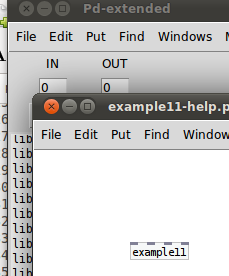
\includegraphics[scale=\Mysize]{example11}
\caption{Vários inlets DSP.}
\label{fig:inlets-dsp}
\end{figure}

% -----+-----+-----+-----+-----+-----+-----+-----+-----+-----+-----+-----+-----+
%      |     |     |     |     |     |     |     |     |     |     |     |     |
% -----+-----+-----+-----+-----+-----+-----+-----+-----+-----+-----+-----+-----+
\section{Primeiro outlet DSP}

A criação dos outlets é feita no construtor do external (veja o exemplo 12) e
é necessário adicionar os outlets à estrutura da classe para que os mesmos
possam ser desalocados quando o objeto for destruído.

\begin{lstlisting}[caption=Criação de outlets DSP]
void * example12_new(void){
   t_example12 *x = (t_example12 *) pd_new(example12_class);

   x->x_outlet_dsp_0 = outlet_new(&x->x_obj, &s_signal);
   x->x_outlet_dsp_1 = outlet_new(&x->x_obj, &s_signal);
   x->x_outlet_dsp_2 = outlet_new(&x->x_obj, &s_signal);
   x->x_outlet_dsp_3 = outlet_new(&x->x_obj, &s_signal);

   return (void *) x;
}
\end{lstlisting}

A definição do método \texttt{\_perform()} será idêntica ao do exemplo
anterior, quando criamos quatro inlets:

\begin{lstlisting}[caption=Método DSP para outlets]
static void example12_dsp(t_example12 *x, t_signal **sp){
   dsp_add(example12_perform, 6, x, sp[0]->s_n, sp[0]->s_vec, sp[1]->s_vec, sp[2]->s_vec, sp[3]->s_vec);
}
\end{lstlisting}

O método perform também será quase idêntico ao do exemplo anterior, porém
recebendo quatro outlets:

\begin{lstlisting}[caption=Método Perform para outlets]
static t_int * example12_perform(t_int *w){
   t_example12 *x = (t_example12 *)(w[1]);
   int n = (int)(w[2]);
   t_float *out1 = (t_float *)(w[3]);
   t_float *out2 = (t_float *)(w[4]);
   t_float *out3 = (t_float *)(w[5]);
   t_float *out4 = (t_float *)(w[6]);
   return (w + 7); // proximo bloco
}
\end{lstlisting}

O resultado pode ser visto na figura \ref{fig:primeiro-outlet}.

\begin{figure}[h!]
\centering
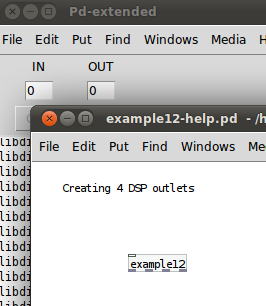
\includegraphics[scale=\Mysize]{example12}
\caption{Primeiro Outlet DSP.}
\label{fig:primeiro-outlet}
\end{figure}

% -----+-----+-----+-----+-----+-----+-----+-----+-----+-----+-----+-----+-----+
%      |     |     |     |     |     |     |     |     |     |     |     |     |
% -----+-----+-----+-----+-----+-----+-----+-----+-----+-----+-----+-----+-----+
\section{Inlets e outlets DSP}

Nosso próximo exemplo (veja o exemplo 13) mistura no mesmo objeto inlets e
outlets DSP, o que é bastante comum.
Neste ponto, deve estar mais ou menos claro como é feita a construção de um
objeto assim.
Neste exemplo, não utilizaremos o primeiro inlet mágico.

\begin{lstlisting}[caption=Criação de vários inlets e outlets DSP]
void * example13_new(void){
   t_example13 *x = (t_example13 *) pd_new(example13_class);

   x->x_inlet_dsp_0 = inlet_new(&x->x_obj, &x->x_obj.ob_pd, &s_signal, &s_signal);
   x->x_inlet_dsp_1 = inlet_new(&x->x_obj, &x->x_obj.ob_pd, &s_signal, &s_signal);
   x->x_inlet_dsp_2 = inlet_new(&x->x_obj, &x->x_obj.ob_pd, &s_signal, &s_signal);
   x->x_inlet_dsp_3 = inlet_new(&x->x_obj, &x->x_obj.ob_pd, &s_signal, &s_signal);

   x->x_outlet_dsp_0 = outlet_new(&x->x_obj, &s_signal);
   x->x_outlet_dsp_1 = outlet_new(&x->x_obj, &s_signal);
   x->x_outlet_dsp_2 = outlet_new(&x->x_obj, &s_signal);
   x->x_outlet_dsp_3 = outlet_new(&x->x_obj, &s_signal);

   return (void *) x;
}
\end{lstlisting}

No método seguinte associamos o método \texttt{\_perform()} à cadeia DSP do
Pure Data:

\begin{lstlisting}[caption=Método DSP para vários inlets e outlets DSP]
static void example13_dsp(t_example13 *x, t_signal **sp){
   dsp_add(example13_perform, 10, x, sp[0]->s_n, sp[0]->s_vec, sp[1]->s_vec, sp[2]->s_vec, sp[3]->s_vec, sp[4]->s_vec, sp[5]->s_vec, sp[6]->s_vec, sp[7]->s_vec);
}
\end{lstlisting}

No método \texttt{\_perform()} recebemos como argumento um bloco de memória
que contém primeiro os buffers de entrada e em seguida os buffers de saída:

\begin{lstlisting}[caption=Método Perform para vários inlets e outlets DSP]
static t_int * example13_perform(t_int *w){
   t_example13 *x = (t_example13 *)(w[1]);
   int n = (int)(w[2]);
   t_float *in1 = (t_float *)(w[3]);
   t_float *in2 = (t_float *)(w[4]);
   t_float *in3 = (t_float *)(w[5]);
   t_float *in4 = (t_float *)(w[6]);
   t_float *out1 = (t_float *)(w[7]);
   t_float *out2 = (t_float *)(w[8]);
   t_float *out3 = (t_float *)(w[9]);
   t_float *out4 = (t_float *)(w[10]);
   return (w + 11); // proximo bloco
}
\end{lstlisting}

Note que não precisamos do inlet ``mágico'' pois este objeto não irá receber
outras mensagens que não sinais de áudio.
Caso queira receber outras mensagens, basta utilizar a macro já apresentada
lembrando que, neste caso, não será necessário adicionar o primeiro inlet.

O resultado pode ser visto na figura \ref{fig:varios-inlets-outlets}.

\begin{figure}[h!]
\centering
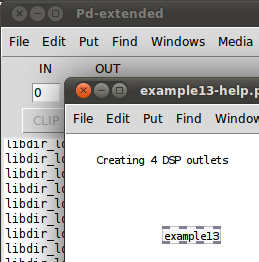
\includegraphics[scale=\Mysize]{example13}
\caption{Vários inlets e outlets DSP.}
\label{fig:varios-inlets-outlets}
\end{figure}

% -----+-----+-----+-----+-----+-----+-----+-----+-----+-----+-----+-----+-----+
%      |     |     |     |     |     |     |     |     |     |     |     |     |
% -----+-----+-----+-----+-----+-----+-----+-----+-----+-----+-----+-----+-----+
\section{Inlets e outlets DSP criados dinamicamente}

Como visto anteriormente, o método DSP passa para o método perform como parâmetro
a quantidade de inlets e outlets.
Por esta razão, a criação dinâmica de inlets e outlets de áudio não é tão simples
quanto a criação dinâmica de inlets e outlets para mensagens.

Ainda assim, é possível definir através de parâmetros para o construtor a
quantidade de inlets e/ou outlets DSP que um external deve possuir.
Isso significa que o número de inlets e outlets é definido dinamicamente,
em tempo de execução, através de um argumento para o construtor, da mesma
maneira que criamos inlets e outlets de mensagens dinamicamente no
capítulo anterior, 

Neste caso, além de armazenarmos a quantidade de canais, armazenaremos na
estrutura da classe um vetor para o sinal de entrada e outro vetor para o sinal
de saída.

\begin{lstlisting}[caption=Estrutura da classe para inlets e outlets DSP dinâmicos]
typedef struct _multigain {
   t_object x_obj;
   t_int count;
   t_float gain;
   t_inlet * x_inlet_gain_float;
   t_sample ** invec;
   t_sample ** outvec;
} t_multigain;
\end{lstlisting}

O construtor cria a quantidade de inlets e outlets passada
como argumento na criação do objeto.
Aqui, poderíamos utilizar \texttt{getbytes()} para alocar o vetor com os dados
de portável.

\begin{lstlisting}[caption=Estrutura do construtor para iolets DSP dinâmicos]
void * multigain_new(t_floatarg count_arg){
   t_multigain *x = (t_multigain *) pd_new(multigain_class);
   x->count = (int)count_arg;
   short i;
   for (i = 0; i < x->count; i++) {
      inlet_new(&x->x_obj, &x->x_obj.ob_pd, &s_signal, &s_signal); // signal inlets
      outlet_new(&x->x_obj, &s_signal);
   }
   x->outvec = getbytes(sizeof(t_sample) * x->count);
   x->invec = getbytes(sizeof(t_sample) * x->count);
   x->x_inlet_gain_float = floatinlet_new(&x->x_obj, &x->gain);
   return (void *) x;
}
\end{lstlisting}

O método DSP irá alocar no próprio objeto os vetores de entrada e saída de DSP e
passar apenas o objeto para o método \texttt{\_perform()}.

\begin{lstlisting}[caption=Método DSP para iolets DSP dinâmicos]
static void multigain_dsp(t_multigain *x, t_signal **sp){
   if(x->count < 1) return;
   int i = 0;
   for(; i < x->count; i++){
      x->invec[i] = getbytes(sys_getblksize() * sizeof(t_sample));
      x->invec[i] = sp[i]->s_vec;
   }
   for(i = 0; i < x->count ; i++){
      x->outvec[i] = getbytes(sys_getblksize() * sizeof(t_sample));
      x->outvec[i] = sp[x->count + i]->s_vec;
   }
   dsp_add(multigain_perform, 2, x, sp[0]->s_n);
}
\end{lstlisting}

A função perform irá, neste exemplo, alterar o ganho dos sinais de entrada,
copiando-os para os sinais de saída.

\begin{lstlisting}[caption=Método Perform para iolets DSP dinâmicos]
static t_int * multigain_perform(t_int *w){
   t_multigain *x = (t_multigain *)(w[1]);
   int n = (int)(w[2]), i = 0, j = 0;
   float gain = x->gain;
   for(; i < x->count ; i++)
      for(j = 0 ; j < n ; j++)
         x->outvec[i][j] = x->invec[i][j] * gain;
   return (w + 3); // proximo bloco
}
\end{lstlisting}

% -----+-----+-----+-----+-----+-----+-----+-----+-----+-----+-----+-----+-----+
%      |     |     |     |     |     |     |     |     |     |     |     |     |
% -----+-----+-----+-----+-----+-----+-----+-----+-----+-----+-----+-----+-----+
\section{Alocação de memória para DSP}

Na introdução da seção de iolets, apresentamos um exemplo (inverter.c) que
modifica um valor recebido.
Como estes parâmetros são passados por referência e não por valor, a modificação
do valor do mesmo irá ser refletida em todos os objetos que recebem esta referência.
No caso de sinais de áudio, não é diferente.

Ao concatenarmos uma série de objetos de áudio, o PD não copia o bloco de áudio
de um para o outro mas utiliza passagem por referência.
Assim, se um objeto altera o bloco recebido, o mesmo será alterado em toda cadeia
de objetos concatenados com o mesmo.

Imaginemos um \external que calcula a mediana de um sinal de
áudio~\footnote{Tal exemplo é real e o \external pode ser encontrado aqui:
\url{http://sourceforge.net/projects/median/}.}.
A maneira mais simples de calcular a mediana é ordenar as amostras e pegar o
valor do meio.
Caso façamos a ordenação no vetor de entrada iremos alterar a ordem das amostras
recebidas e todos os objetos conectados a este sinal receberão o mesmo com as
amostras ordenadas.
Por esta razão, é importante verificar se podemos ou não alterar o valor de um
vetor de amostras recebidos.

\section{Outras funcionalidades para DSP}

Vários processamentos em sinais dependem da taxa de amostragem, tamanho de bloco
e quantidade de canais de entrada e saída.
Para acessar estas informações no PD, utilizamos duas funções da API:

\begin{itemize}
\item \texttt{int sys\_getblksize(void);}
   Retorna o tamanho do bloco de processamento do Pure Data.
\item  \texttt{t\_float sys\_getsr(void);}
Retorna qual a amostragem (Sample Rate) atual do Pure Data.
\item \texttt{int sys\_get\_inchannels(void);}
Retorna a quantidade de canais de entrada do Pure Data.
\item \texttt{int sys\_get\_outchannels(void);}
Retorna a quantidade de canais de saída do Pure Data.
\end{itemize}

Estas e outras funções podem ser encontradas no último capítulo deste tutorial.
